\documentclass[a4paper,12pt]{article}
\usepackage[top = 2.5cm, bottom = 2.5cm, left = 2.5cm, right = 2.5cm]{geometry}
\usepackage[T1]{fontenc}
\usepackage[utf8]{inputenc}
\usepackage{multirow} 
\usepackage{booktabs} 
\usepackage{graphicx}
\usepackage[spanish]{babel}
\usepackage{setspace}
\setlength{\parindent}{0in}
\usepackage{float}
\usepackage{fancyhdr}
\usepackage{amsmath}
\usepackage{amssymb}
\usepackage{amsthm}
\usepackage[numbers]{natbib}
\newcommand\Mycite[1]{%
	\citeauthor{#1}~[\citeyear{#1}]}
\usepackage{graphicx}
\usepackage{subcaption}
\usepackage{booktabs}
\usepackage{etoolbox}
\usepackage{minibox}
\usepackage{hyperref}
\usepackage{xcolor}
\usepackage[normalem]{ulem}
 \useunder{\uline}{\ul}{}
\usepackage[skins]{tcolorbox}
%---------------------------

\newtcolorbox{cajita}[1][]{
	 #1
}

\newenvironment{sol}
{\renewcommand\qedsymbol{$\square$}\begin{proof}[\textbf{Solución.}]}
	{\end{proof}}

\newenvironment{dem}
{\renewcommand\qedsymbol{$\blacksquare$}\begin{proof}[\textbf{Demostración.}]}
	{\end{proof}}

\newtheorem{problema}{Problema}
\newtheorem{definicion}{Definición}
\newtheorem{ejemplo}{Ejemplo}
\newtheorem{teorema}{Teorema}
\newtheorem{corolario}{Corolario}[teorema]
\newtheorem{lema}[teorema]{Lema}
\newtheorem{prop}{Proposición}
\newtheorem*{nota}{\textbf{NOTA}}
\renewcommand\qedsymbol{$\blacksquare$}
\usepackage{svg}
\usepackage{tikz}
\usepackage[framemethod=default]{mdframed}
\global\mdfdefinestyle{exampledefault}{%
linecolor=lightgray,linewidth=1pt,%
leftmargin=1cm,rightmargin=1cm,
}




\newenvironment{noter}[1]{%
\mdfsetup{%
frametitle={\tikz\node[fill=white,rectangle,inner sep=0pt,outer sep=0pt]{#1};},
frametitleaboveskip=-0.5\ht\strutbox,
frametitlealignment=\raggedright
}%
\begin{mdframed}[style=exampledefault]
}{\end{mdframed}}
\newcommand{\linea}{\noindent\rule{\textwidth}{3pt}}
\newcommand{\linita}{\noindent\rule{\textwidth}{1pt}}

\AtBeginEnvironment{align}{\setcounter{equation}{0}}
\pagestyle{fancy}

\fancyhf{}









%----------------------------------------------------------
\lhead{\footnotesize Geometría Moderna}
\rhead{\footnotesize  Rudik Roberto Rompich}
\cfoot{\footnotesize \thepage}


%--------------------------

\begin{document}
 \thispagestyle{empty} 
    \begin{tabular}{p{15.5cm}}
    \begin{tabbing}
    \textbf{Universidad del Valle de Guatemala} \\
    Departamento de Matemática\\
    Licenciatura en Matemática Aplicada\\\\
   \textbf{Estudiante:} Rudik Roberto Rompich\\
   \textbf{Correo:}  \href{mailto:rom19857@uvg.edu.gt}{rom19857@uvg.edu.gt}\\
   \textbf{Carné:} 19857
    \end{tabbing}
    \begin{center}
        MM2031 - Geometría Moderna - Catedrático: María Eugenia Contreras Pinillos\\
        \today
    \end{center}\\
    \hline
    \\
    \end{tabular} 
    \vspace*{0.3cm} 
    \begin{center} 
    {\Large \bf  HT 1
} 
        \vspace{2mm}
    \end{center}
    \vspace{0.4cm}
%--------------------------

\begin{problema}
	Dos circunferencias se intersecan en los puntos $A$ y $B$. Sea $l$ una recta cualquiera que pasa por el punto $A$ interceptando  las circunferencias en los puntos $P$ y $Q$. Sea $R$ un punto que divide el segmento $PQ$ en una razón constante.  Demuestre que el lugar geométrico para $R$ es una circunferencia.
	\begin{figure}[H]
		\centering
		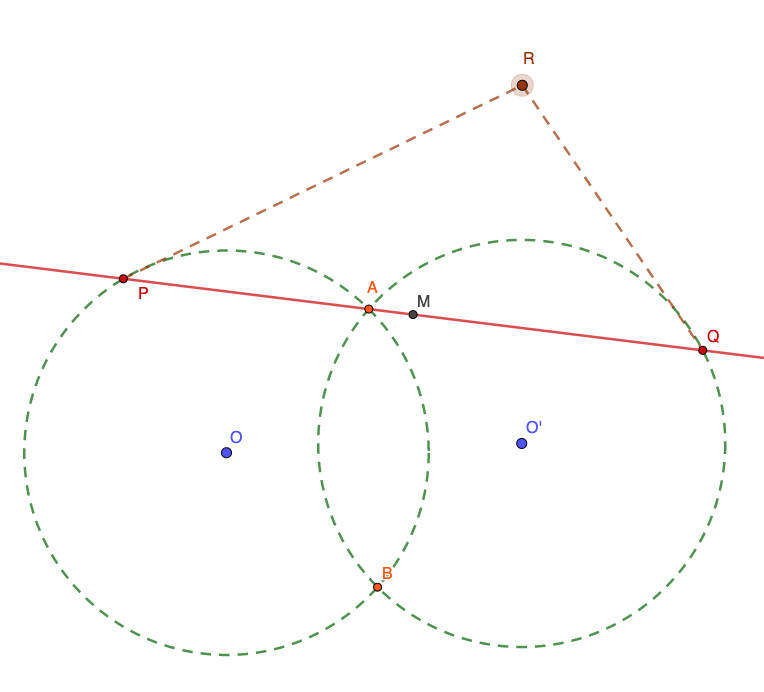
\includegraphics[scale=0.3]{Images/1}
		\caption{Construcción}
	\end{figure}
\end{problema}
\begin{cajita}
	El círculo de Apolonio no se puede usar ya que $P$ y $Q$ no son fijos. \end{cajita}
\begin{dem}
	Por hipótesis, tenemos que los círculos con centros $O$ y $O'$ respectivamente se intersectan en $A$ y $B$; también $l$ es una recta que intersecta a $P$ y $Q$ y tenemos que 
	
	\begin{gather}
		\frac{RP}{RQ}=k\implies \frac{RP^2}{RQ^2}=k^2\implies RP^2 = k^2 RQ^2.
	\end{gather}

	Supóngase que $M$ es el punto medio de $PQ$ y sin pérdida de generalidad, asumamos que está ubicado en $(0,0)$ (En caso contrario, tendríamos que hacer probablemente una parametrización que incluya la ubicación de $O$ y $O'$...) $\implies PM=MQ=m$ tal que $P(-m,0)$ y $Q(0,m)$. Por otra parte $R$ se encuentra en un punto cualesquiera, $R(x,y)$. $\implies$ Considerando (1) tenemos: 
	\begin{align*}
		(x-m)^2+y^2 &= k^2 \left[(x+m)^2+y^2\right]\\
		x^2 -2xm +m^2 +y^2&=x^2k^2+2xmk^2 +m^2k^2  +y^2k^2\\
		x^2 -2xm +m^2 +y^2-x^2k^2-2xmk^2 -m^2k^2  -y^2k^2&= 0\\
		x^2(1-k^2)+y^2(1-k^2)-2mx(1+k^2)+m^2(1-k^2)&= 0 \qquad (\textcolor{red}{\div(1-k^2)})
	\end{align*}	
Entonces, tenemos
$$x^2+y^2 - \frac{2mx(1+k^2)}{1-k^2}+m^2=0,$$
la cual es la ecuación del círculo y por lo tanto el punto geométrico de $R$ es un círculo. 
\end{dem}

\begin{problema}
	Sea $A$ un punto cualesquiera de la circunferencia de similitud de dos circunferencias cuyos centros son $O$ y $O'$. Dibujar $AO$, y en ella obtener $AO''=k AO'$. Utilizando a  $O''$ como centro, dibujar una circunferencia cuyo radio es k veces el de la circunferencia $O'$. Estas circunferencias $O$ y $O''$ son homotéticas con $A$ como centro de similitud.
	\begin{figure}[H]
		\centering
		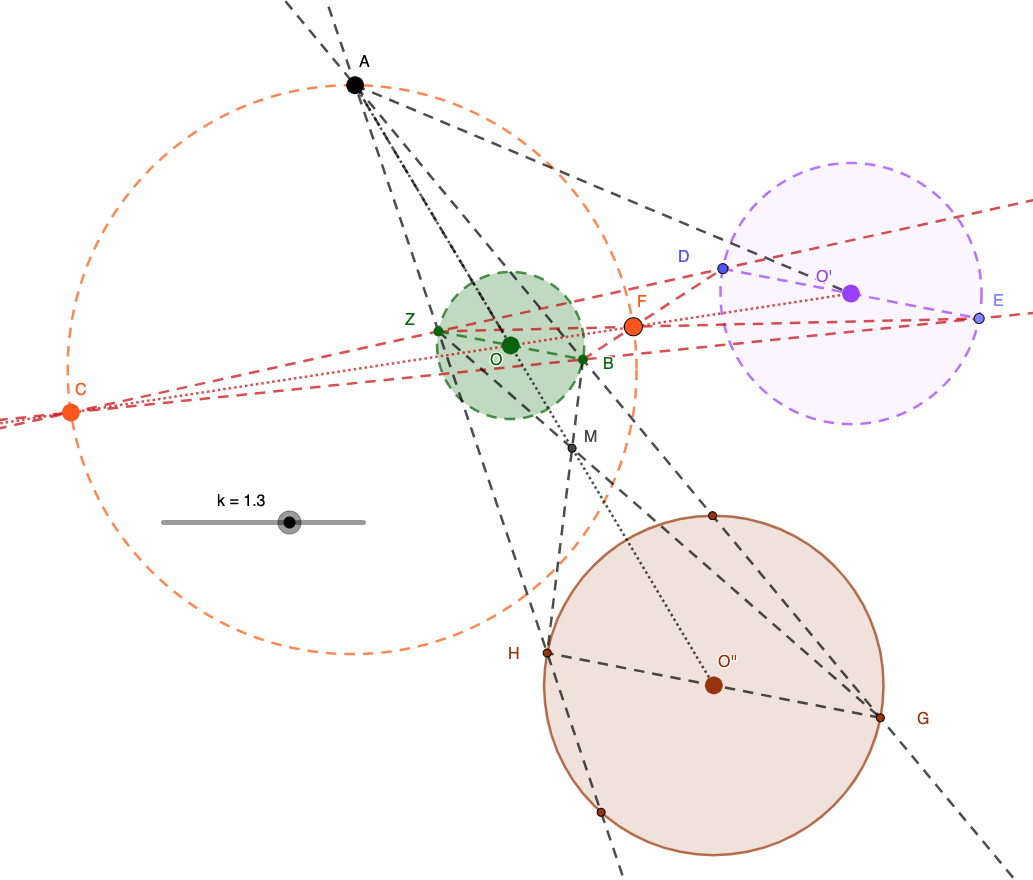
\includegraphics[scale=0.3]{Images/2}
		\caption{Construcción}
	\end{figure}
\end{problema}
\begin{dem}
	Por hipótesis, sabemos que $AO''=k AO'$ está sobre $AO$ y tenemos el circulo con $O''$ como centro y $k\cdot EO'$ como radio. Ahora bien, demostraremos que las dos circunferencias son homotéticas, sea $HG\parallel ZB$ en donde $HZ$  y  $HB$ interceptan los puntos $A$ y $M$ respectivamente. $\implies$ Por el teorema de paralelas y transversas $\angle BOM \cong \angle HO''M\implies$ Por ángulos verticales $O'' M H \cong OMB \implies \triangle MBO \sim  \triangle ZMB$.  $\implies$ La circunferencias con centros $O$ y $O''$ son homotéticas donde $A$ y $M$ son los centros de similitud. 
\end{dem}

\begin{problema}
	$P$ y $P'$ son dos puntos antihomólogos de dos circunferencias cuyos centros son $O$ y $O'$ respectivamente, y $A$ es el centro de similitud que está en $PP'$. Determine si los triángulos $APO$ y $AP'O'$ son semejantes.
	\begin{figure}[H]
		\centering
		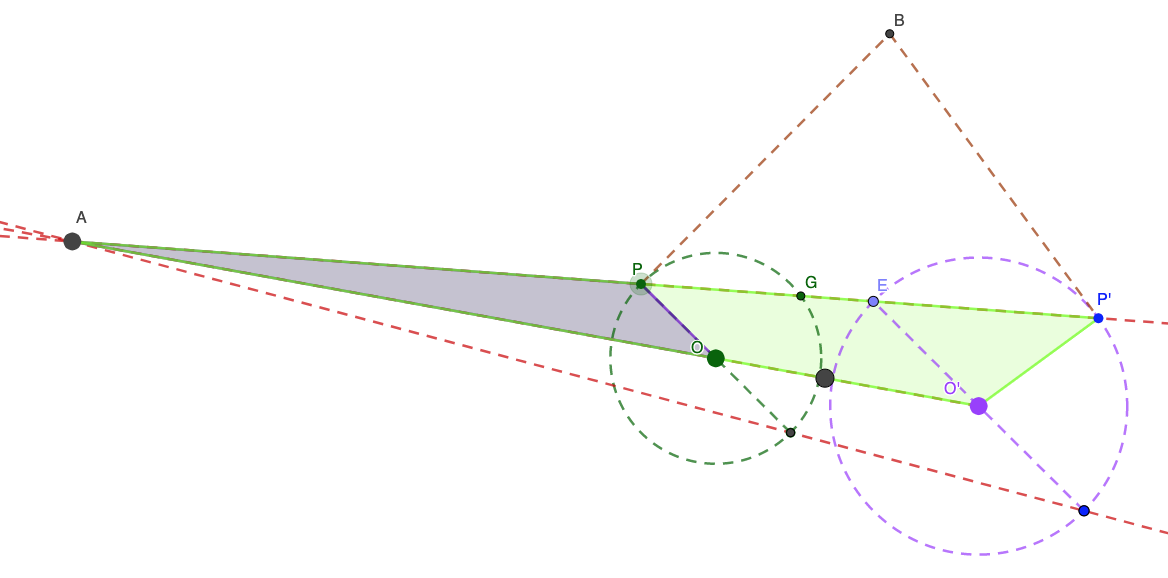
\includegraphics[scale=0.3]{Images/3}
		\caption{Construcción}
	\end{figure}
\begin{dem}
	Por hipótesis, $P$ y $P'$ son dos puntos antihomólogos de dos circunferencias cuyos centros son $O$ y $O'$ respectivamente, y $A$ es el centro de similitud que está en $PP'$. Por reducción al absurdo, supóngase que $\triangle APO$ y $\triangle AP'O'$ son semejantes. Es decir, 
	$$\angle PAO \cong P'AO', \angle AOP\cong \angle AO'P' \quad \text{y} \quad\angle OPA\cong \angle O'P'A.$$
	
	$\implies$ Por la construcción de los puntos antihomólogos tenemos $OP\parallel O'E$. Además, se propuso que $BP$ y $P'B$ son  tangentes a $P'$ y $P$, respectivamente tal que por teorema tenemos $\angle BPP' \cong \angle PP'B$. $\implies$ Por la definición de tangente, 
	\begin{align}
		\angle PP'B + \angle O'P'A =90^\circ
		\intertext{y}
		\angle BPP' + \angle P'PO =90^\circ
	\end{align} 
De (1) se tiene que $\underbrace{\angle BPP'}_{\cong \angle PP'B}+\underbrace{\angle OPA}_{\cong \angle O'P'A} =90^\circ$ e igualando con (2) tenemos 
\begin{gather}
	\angle BPP'+\angle OPA = \angle BPP' + \angle P'PO 
\end{gather}
$\implies \angle OPA = \angle P'PO $. Sin embargo, nótese que $\angle OPA+ \angle P'PO = 180^\circ\implies \angle OPA = \angle P'PO = 90^\circ \implies $ Tomando en cuenta (1) y (2) tenemos $\angle BPP' \cong \angle PP'B = 0^\circ $. Pero eso implicaría que $P$ y $P'$ no son puntos antihomólogos ($\to\gets$). 
\begin{figure}[H]
	\centering
	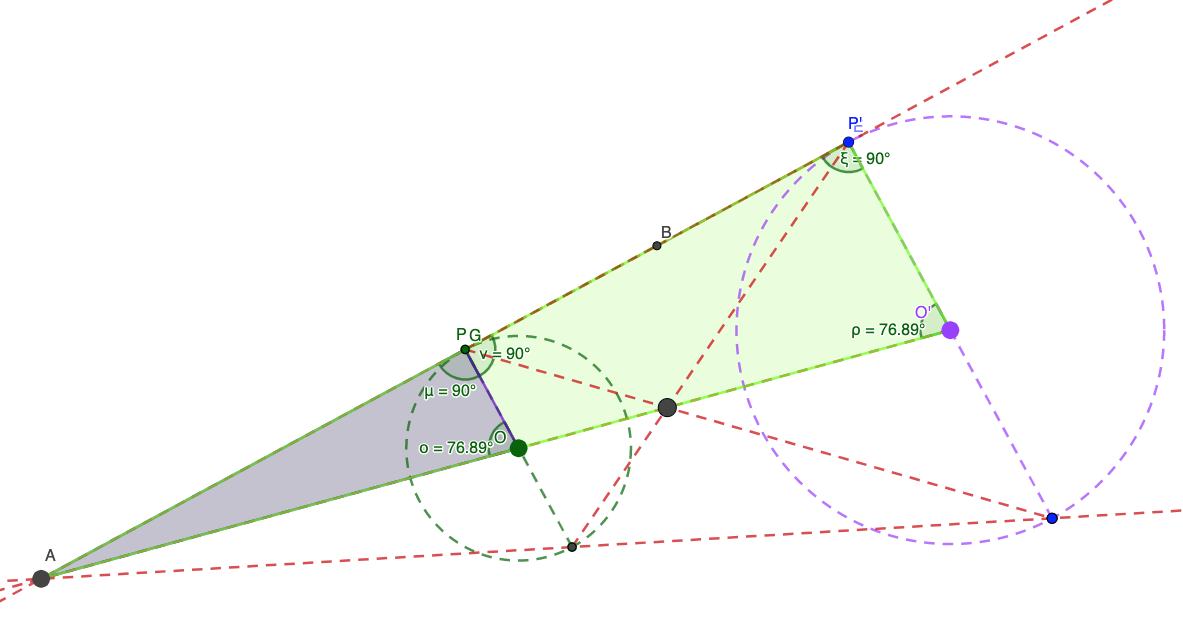
\includegraphics[scale=0.2]{Images/3a}
	\caption{Contradicción - Caso especial}
\end{figure}

Por lo tanto, $\triangle APO$ y $\triangle AP'O'$ no son semejantes. 
\end{dem}
\end{problema}


\begin{problema}
	Si una circunferencia corta los lados $BC$, $CA$ y $AB$ del triángulo $ABC$ en los puntos $P$, $P'$, $Q$, $Q'$, $R$, $R'$ respectivamente, y si $AP, BQ$ y $CR$ son concurrentes, entonces $AP'$, $BQ'$, y $CR'$ también son concurrentes.
		\begin{figure}[H]
		\centering
		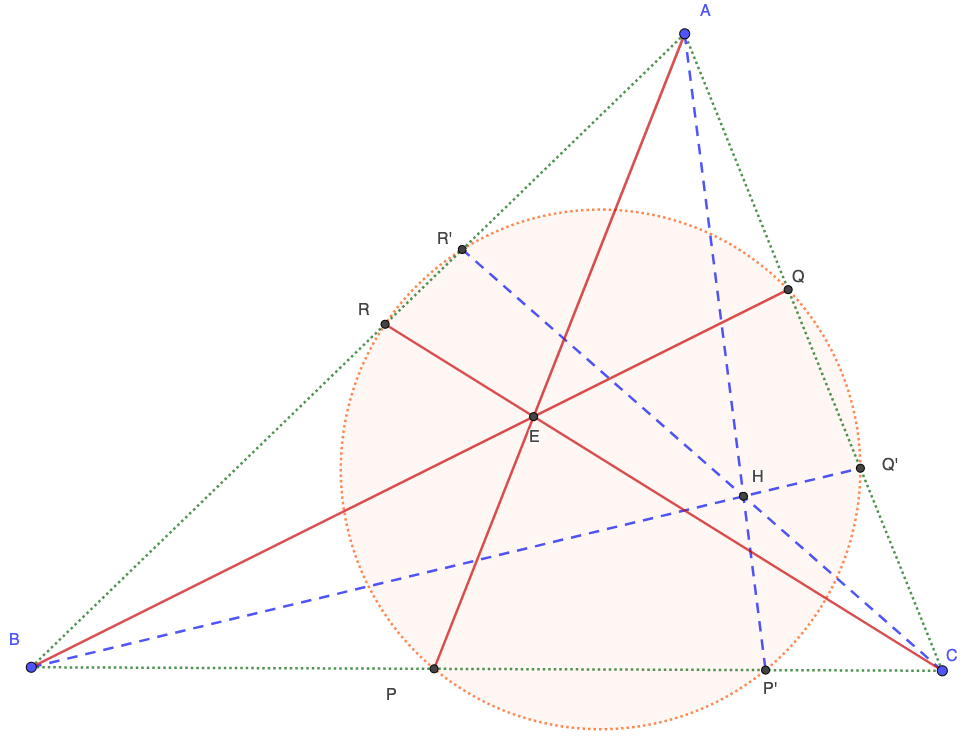
\includegraphics[scale=0.3]{Images/4}
		\caption{Construcción}
	\end{figure}
	
\end{problema}


\begin{dem}
	Por hipótesis, una circunferencia corta los lados $BC$, $CA$ y $AB$ del triángulo $ABC$ en los puntos $P$, $P'$, $Q$, $Q'$, $R$, $R'$ respectivamente, además 
	$$AP\cap BQ \cap CR,$$
	
	que se intersectan en $E$. Por el teorema de Ceva, la siguiente igualdad se cumple: 
	\begin{gather}
		\frac{AR}{RB}\cdot\frac{BP}{PC}\cdot\frac{CQ}{QA} =1.
	\end{gather}
	
	$\implies$ 
	Sean $P',Q'$ y $R'$ puntos que están en $BC$, $CA$ y $AB$ del $\triangle ABC$. 	$\implies$  Por lo anterior, la siguiente igualdad se cumple
	
	$$\frac{AR'}{R'B}\cdot\frac{BP'}{P'C}\cdot\frac{CQ'}{Q'A} =1. $$
	
	Por lo tanto, por el teorema de Ceva $AP'\cap BQ' \cap CR'$. 
\end{dem}



%---------------------------
\bibliographystyle{apa}
\bibliography{referencias.bib}

\end{document}